\documentclass{article}


\usepackage{hw_style}
\usepackage{enumerate}
\usepackage{graphicx}
\usepackage{verbatim}

% Homework Specific Information
\newcommand{\hmwkTitle}{Homework \#5}
\newcommand{\hmwkDueDate}{Tuesday, June 26, 2012, 9:00AM}
\newcommand{\hmwkAuthorName}{Kurt Rudolph}%Name:
\newcommand{\hmwkNetID}{rudolph9}%your netid
\newcommand{\hmwkNotes}{}%I worked with...

\newcommand{\hmwkSubTitle}{}
\newcommand{\hmwkClass}{Math 461}
\newcommand{\hmwkClassTime}{}
\newcommand{\hmwkClassInstructor}{Kenneth B. Stolarsky}

\begin{document}
\begin{spacing}{1.1}
\maketitle

%=============================p.107 66==========================% 
\newpage
\begin{homeworkProblem}
The probability of the closing of the $i$th relay in the circuits 
shown in Figure 3.4 is given by $p_i, i = 1, 2, 3, 4, 5$. If all 
relays function independently, what is the probability that a 
current flows between $A$ and $B$ for the respective circuits?
Hint for (b): Condition on whether relay 3 closes.

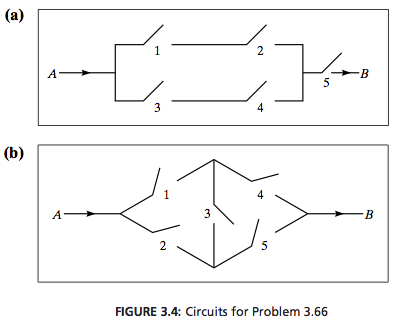
\includegraphics{p108_66}
  \begin{enumerate}[(a)]
    \item
      \begin{homeworkSection}{Solution}
        \[P(A) = p_5 (p_1 p_2 + p_3 p_4)\]
      \end{homeworkSection}
    \item
      \begin{homeworkSection}{Solution}
        \[P(B) = p_1 p_5 + p_1 p_3 p_5 + p_2 p_5 + p_2 p_3 p_4\]
      \end{homeworkSection}
  \end{enumerate}
\end{homeworkProblem}
%=============================p.173 5==========================% 
\newpage
\begin{homeworkProblem}
  Let $X$ represent the difference between the number of heads
  and the number of tails obtained when a coin is tossed $n$ times. 
  What are the possible values of $X$?
  \begin{homeworkSection}{Solution}
    Assuming the absolute value to be taken of the difference and
    letting $i$ represent the possible values, then 

    \[0 \le i \le n\]

  \end{homeworkSection}
\end{homeworkProblem}
%=============================p.173 6==========================% 
\newpage
\begin{homeworkProblem}
In Problem 5, for $n = 3$, if the coin is assumed fair, what are 
the probabilities associated with the values that $X$ can take on?
  \begin{homeworkSection}{Solution}
    Following our proof from problem 5, we find $X_i$ where 
    $0 \le i \le n$.
    \begin{itemize}
      \item $\{X_0\} = \emptyset$
      \item $\{X_1\} = [tth, tht, htt, hht, hth, thh]$
      \item $\{X_2\} = \emptyset$
      \item $\{X_3\} = [hhh,ttt]$
    \end{itemize}
    Where,
    \begin{itemize}
      \item $P( \{X_0\}) = \emptyset$
      \item $P( \{X_1\}) = \frac{ 6}{ 8} = \frac{ 3}{ 4}$
      \item $P( \{X_2\}) = \emptyset$
      \item $P( \{X_3\}) = \frac{ 2}{ 8} = \frac{ 1}{ 4}$
    \end{itemize}
  \end{homeworkSection}
\end{homeworkProblem}
%=============================p.173 21==========================% 
\newpage
\begin{homeworkProblem}
  Four buses carrying 148 students from the same school arrive at 
  a football stadium. The buses carry, respectively, 40, 33, 25, 
  and 50 students. One of the students is randomly selected. 
  Let $X$ denote the number of students that were on the bus carrying 
  the randomly selected student. One of the 4 bus drivers is also 
  randomly selected. Let $Y$ denote the number of students on her bus.


  \begin{homeworkSection}{Definitions}

    Given
      \begin{itemize}
        \item $E[ X] = \sum\limits_{x:p( x) > 0}{ x p( x)}$
      \end{itemize}
    Let
      \begin{itemize}
        \item $S$ be the set of students, where $|S| = 148$
        \item $s_i \in S$, where $1 \le i \le 148$
        \item $B$ be set of buses, where $|B| = 4$
        \item $b_i \in B$, where $1 \le i \le 4$
        \item $|b_i|$ denote the number of students on bus $i$
          \begin{itemize}
            \item $|b_1| = 40$
            \item $|b_2| = 33$
            \item $|b_3| = 25$
            \item $|b_4| = 50$
          \end{itemize}
        \item $BD$ be the set of bus drivers where $1 \le i \le 4$
        \item $s_X$ be the randomly selected student.
        \item $bd_Y$ be the randomly selected bus driver.
        \item $b_X$ be the bus which the randomly selected student is on.
        \item $b_Y$ be the bus the randomly selected bus driver drives.
      \end{itemize}
  \end{homeworkSection}
  \begin{enumerate}[(a)]
    \item Which of $E[ |X|]$ or $E[ |Y|]$ do you think is larger? Why?
      \begin{homeworkSection}{Solution}
        I believe $E[ |X|] < E[ |Y|]$.  My reason follows that since the 
        probability a student will be selected from a bus carrying more students 
        over a bus carrying less students.  
        Since the probability that a bus driver will be selected carry a bus with a large
        number of students is equal to a bus driver being selected from a bus carrying
        a small number of students.
      \end{homeworkSection}
    \item Compute $E[ |X|]$ and $E[ |Y|]$?
      \begin{homeworkSection}{Solution}
        \begin{itemize}
          \item $E[ |X|] = (|b_1|) P( b_1) + (|b_2|) P( b_2) + (|b_3|) P( b_3) + (|b_4|) P( b_4)$
          \item $E[ |Y|] = (|bd_1|) P( bd_1) + (|bd_2|) P( bd_2) + (|bd_3|) P( bd_3) + (|bd_4|) P( bd_4)$
        \end{itemize}

      \end{homeworkSection}
  \end{enumerate}
\end{homeworkProblem}
\end{spacing}
\end{document}

\begin{comment}%==========================================================
%=============================Problemi==========================% 
\newpage
\begin{homeworkProblem}

  \begin{homeworkSection}{Solution}

  \end{homeworkSection}
\end{homeworkProblem}
%=============================Problemi==========================% 
\begin{homeworkProblem}

  \begin{enumerate}[(a)]
    \item 
      \begin{homeworkSection}{Solution}

      \end{homeworkSection}
  \end{enumerate}
\end{homeworkProblem}
\end{comment}

\begin{comment}
  ## Homework
Due Tuesday
* P.107 66
* P.173 5, 6, 21, 35, 37, 38
* P.180 6, 7, 8, 9
\end{comment}
